%---------------------------------------------------------------------
%
%                          Cap�tulo 5
%
%---------------------------------------------------------------------

\chapter{Implementation Study}

\begin{FraseCelebre}
\begin{Frase}
Time of your life
\end{Frase}
\begin{Fuente}
Thomas \& Guy-Manuel, Daft Punk
\end{Fuente}
\end{FraseCelebre}


\begin{resumen}
In this chapter, tasks related to the physical implementation of the platform are described. These tasks cover from the layout design, 3D modeling, and GERBER files generation, to the final components mounting on the PCB. Decisions about components or layout designs, and final results are exposed.  
\end{resumen}



%-------------------------------------------------------------------
\section{Introduction}
%-------------------------------------------------------------------
\label{cap5:sec:introduction}
%------------------------------------------------------------------

Once the system is designed over a logic circuitry level, it is moment to build a \ac{PCB} design responsive to the developed schematics. This process includes the PCB dimensions, components placement, tracks routing, silkscreens, etc. These tasks are achieved over the Altium Designer, same software described in Section \ref{cap4:sub:altiumDesigner}.

All the implementations share some common features regarding their layout designs. On the one hand, the used components will keep, whenever possible\footnote{Some components do not offer \ac{SMD} packaging due to their electric properties.}, \ac{SMD} packaging. This technology gives a more reduced size and supports lower power ratings. Precisely, the \ac{SMD} package used for most of two-terminal components is the 0603 size\footnote{1.6 mm x 0.8 mm (0.063 in x 0.031 in). Typical power rating for resistors are 0.1 watt.}

All the created layouts are built over two-layer boards. Two layers are enough for our purposes since they allow to place the components in a sufficiently reduced area and power planes are not required. More layers, in addition, would increase significantly the board costs. 

For the tracks routing process, some considerations are taken. Ground planes are placed to face noise reduction, this way a low impedance way is provided for the power signals. Moreover, parasitic \ac{EM} emissions are reduced. Power tracks are width enough to support the supplied current flow.

Together with the layout deployment, Altium Designer offers the chance to embed 3D models of each component, building up eventually a whole 3D model of the complete board. This tool was employed, and 3D models were rendered, obtaining a preview of the modules on advance to their materialization.

\ac{PCB} manufacturer, PCBCART\footnote{www.pcbcart.com} will produce the \ac{PCB}s from the outputted fabrication files. Final \ac{PCB} posses a 1.6 mm thickness, and copper layers are 35 $\mu$m thick. 

Sequential mounting, and the existing firmware allow to carry through simple tests to check proper functionality and detect errors. Actually, several corrections and adjustments were made during the mounting task.  

%-------------------------------------------------------------------
\subsection{Tools}
%-------------------------------------------------------------------
Small package components, like the employed here, requires for precision tools to be mounted. Proper tweezers are helpful dealing with tiny components. The soldering station used is a JBC AM 6000\cite{jbc}, offering several soldering tips on the 1-4 mm diameter and useful tools as hot tweezers or desoldering accessories. Microscope is very valuable for better precision, the one used is a Bausch \& Lomb StereoZoom 4 Microscope. 

Components use to include at their datasheets guidelines about their surrounding layout, soldering tips, or mounting processes. They are reviewed and taken into account for the process.

%-------------------------------------------------------------------
\section{Transceivers - $\mu$Trans 434/868}
%-------------------------------------------------------------------
\label{cap5:sec:transceivers}
%------------------------------------------------------------------

\begin{figure}[!h]
        \centering
		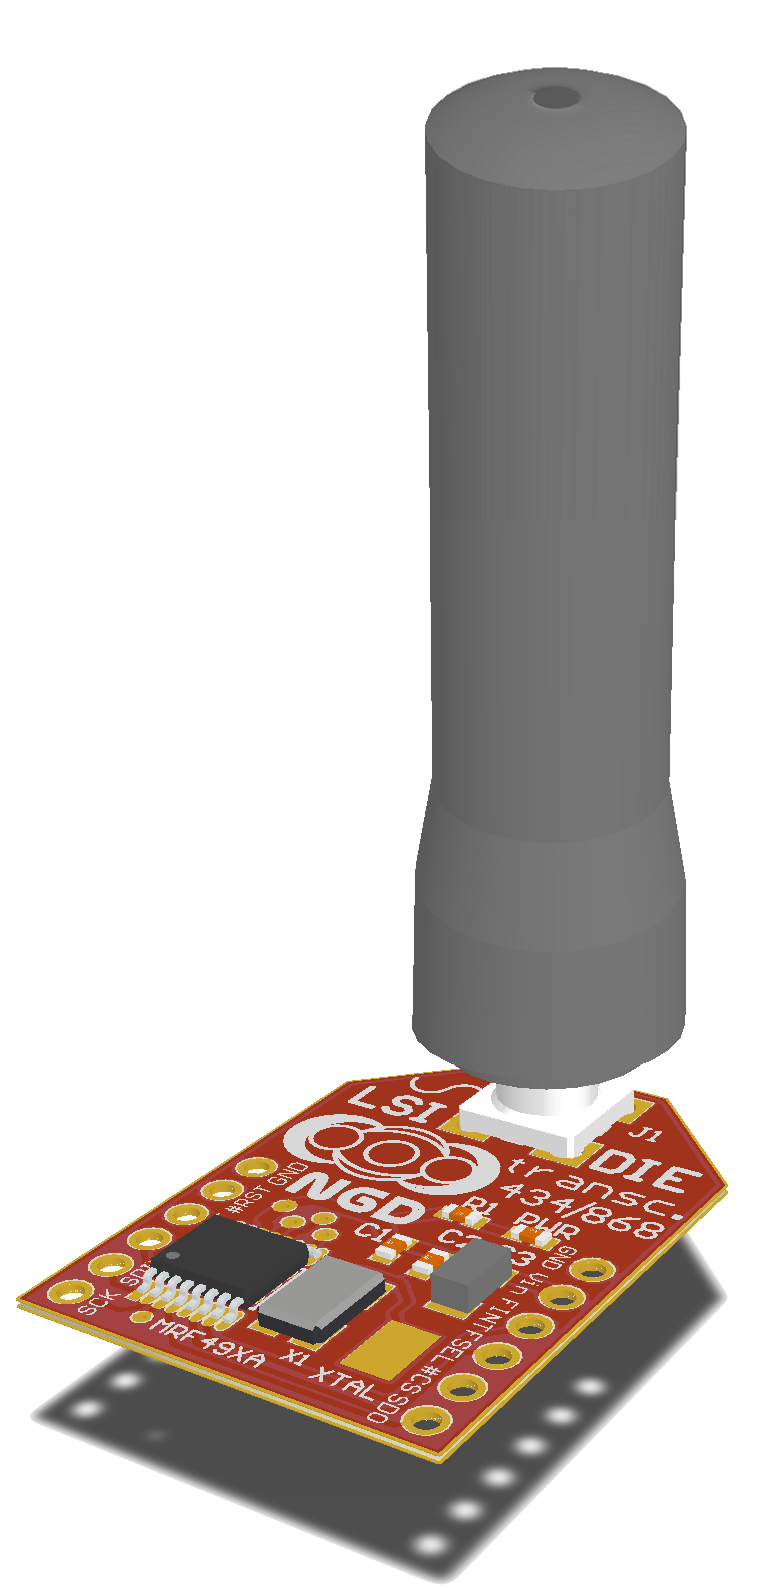
\includegraphics[width=0.3\textwidth]{Imagenes/Bitmap/Capitulo5/mtrans3d}  
        \caption{$\mu$Trans 434/868 3D model.}
        \label{fig:cap5:mtrans3dmodel}
\end{figure}

%-------------------------------------------------------------------
\subsection{Description}
%-------------------------------------------------------------------

As it was viewed, this module was developed because of the non-existence of reduced size \ac{RI}s including the MRF49XA transceiver. Therefore, by definition, the module must posses a reduced size. Taking advantage of the included MRF24j40MA \ac{RI}, it was decided to design a \ac{PCB} module fitting the footprint of the named \ac{RI}. This way a single footprint is common to all the included \ac{RI}s. This footprint is defined in Figure \ref{fig:cap5:realsizemtrans}.


\begin{figure}[!h]
\centering

\subfloat[$\mu$Trans 434/868 and MRF24j40MA footprint. 20.5x28.1 mm.]{\label{fig:cap5:mtransfootprint}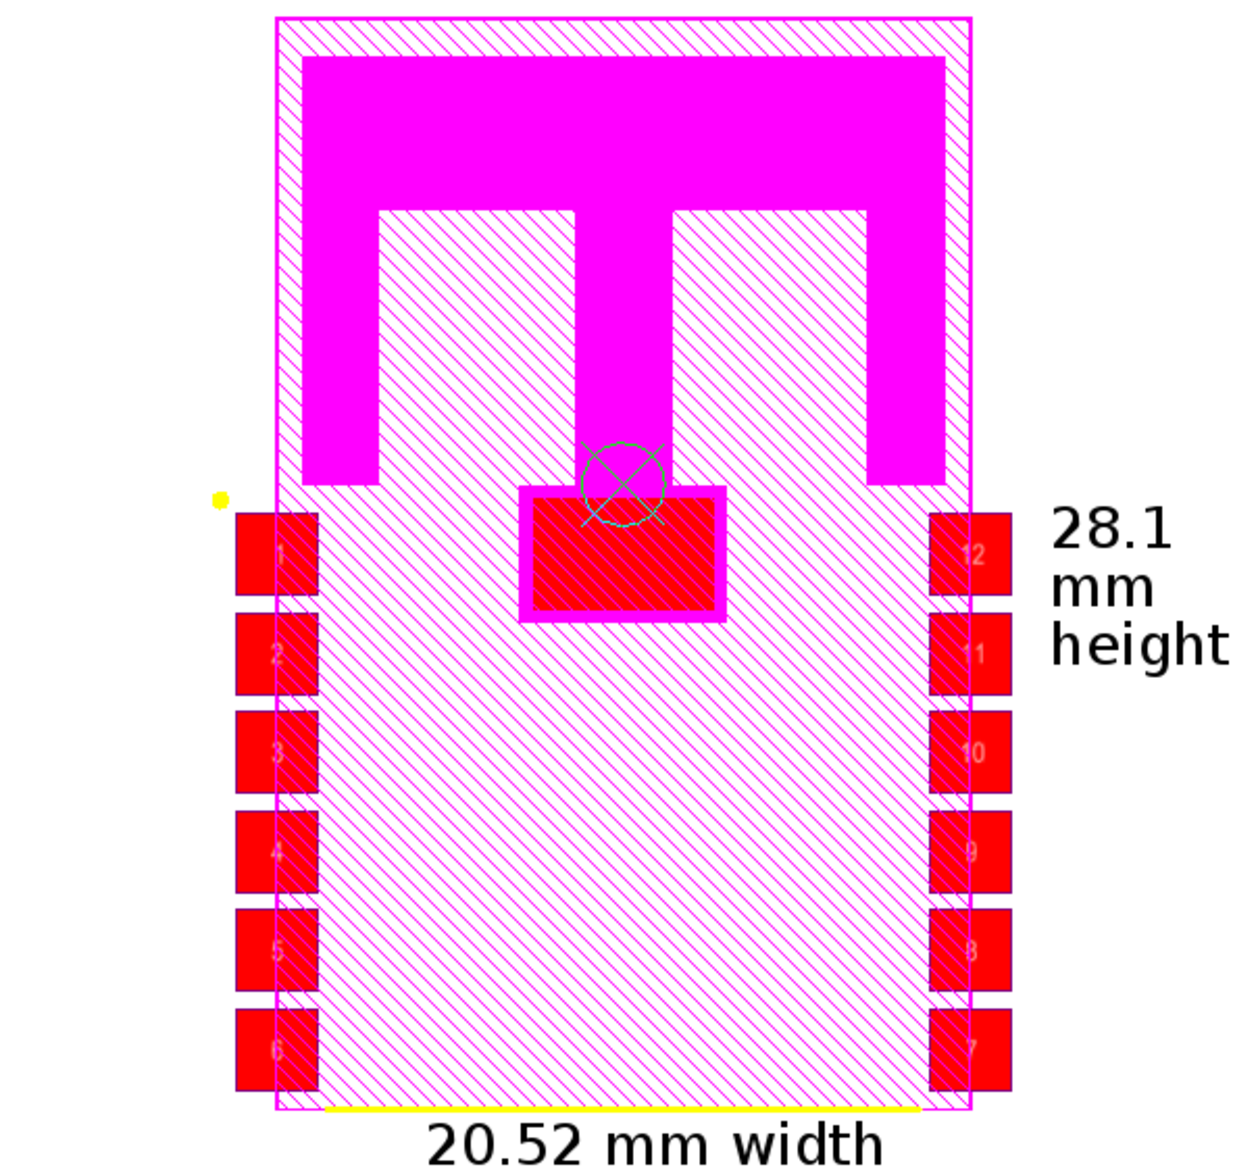
\includegraphics[height=107px]{Imagenes/Vectorial/Capitulo5/transfootprint}}%
\qquad
\subfloat[$\mu$Trans 434/868 PCB shape. 20.8x30 mm.]{\label{fig:cap5:mtransshape}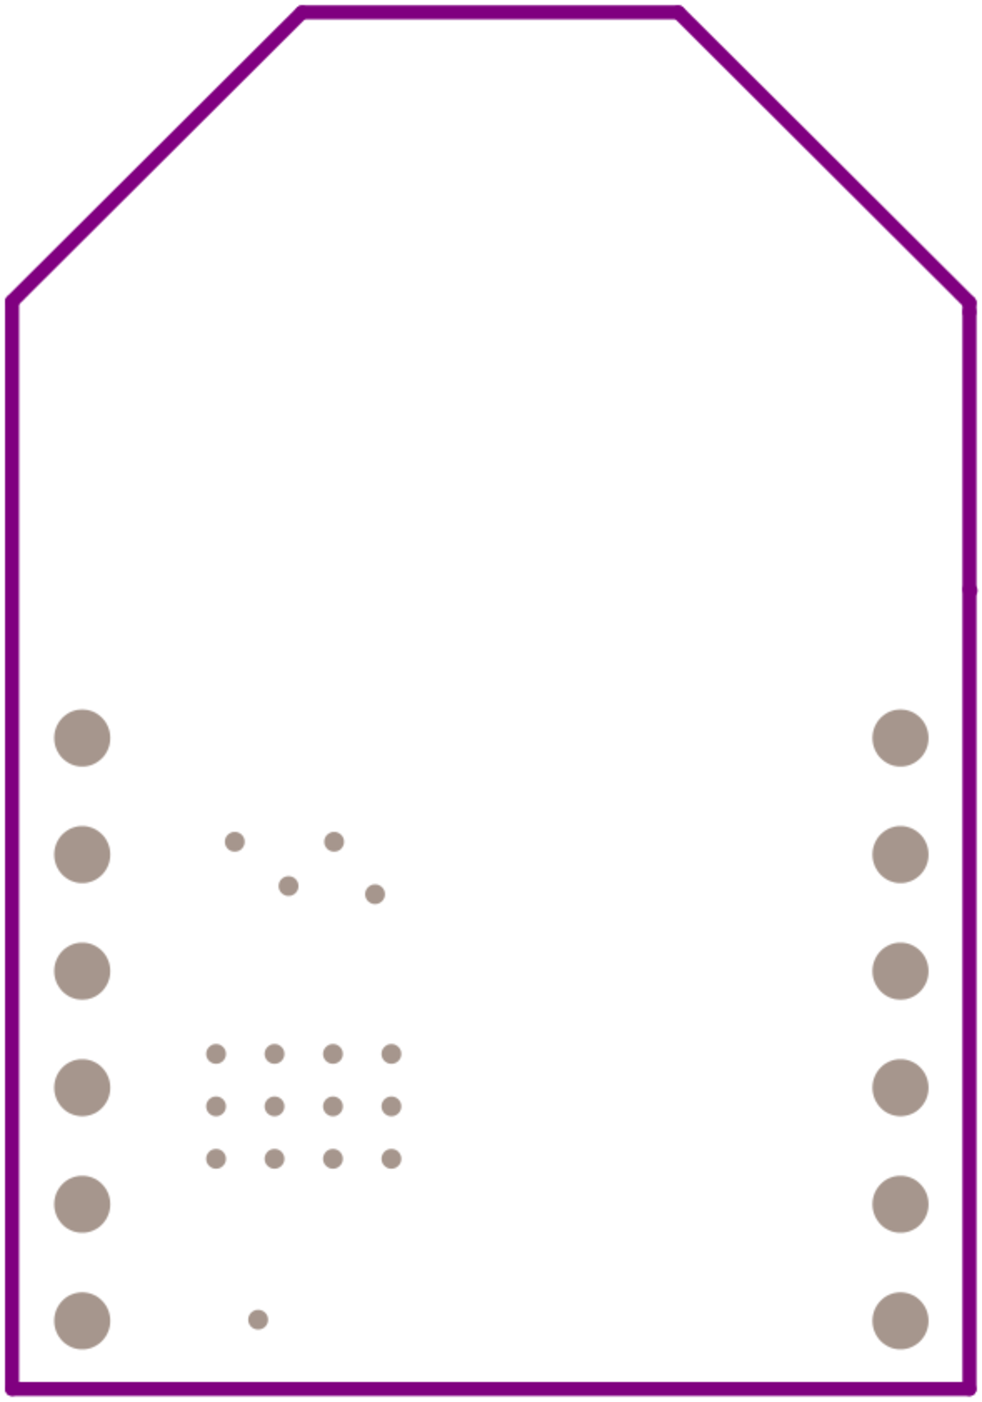
\includegraphics[height=115px]{Imagenes/Vectorial/Capitulo5/mtransshape}}%

\caption{Real size footprint and shape for $\mu$Trans module.}
\label{fig:cap5:realsizemtrans}

\end{figure}

The \ac{PCB} size must be suitable for this footprint, not exceeding its width. $\mu$Trans \ac{PCB} shape is defined as in Figure \ref{fig:cap5:realsizemtrans}.

Module pads are based vias\footnote{A via is a electrical connection between layers in a physical electronic circuit that goes through the plane of one or more adjacent layers.}, with a 1.2 mm diameter through hole. These holes are width enough to let the solder tip into them and solder the pads over the footprint. These pads constitute the electrical interface between the $\mu$Trans and \ac{CNGD} and suppose a low-cost and size solution.  

MRF49XA datasheet provides hints for the inclusion of the transceiver into a \ac{PCB}. It recommends to fill with ground vias the area underneath the transceiver. In addition, to have an easily accessible measure of the clock signal, the top layer posses a small pad that provides this signal. Minimal clearance among tracks is set to 0.2 mm and the standard track width is 0.2 mm. Power tracks width is set to 0.4 mm and ground planes are placed on top and bottom layers. Vias through holes minimal diameter are 0.4 mm width. Table \ref{tab:ap2:mtranscomponents} at the Appendix \ref{ap2:layouts} contains the needed components for the $\mu$Trans 434/868 on both versions.

The 
**** COAXIAL
****************** ANTENA

%-------------------------------------------------------------------
\subsection{Layout}
%-------------------------------------------------------------------
Different layers of the layout can be observed at Appendix \ref{ap2:layouts}. Figures \ref{ap2:mtranstop} and \ref{ap2:mtransbottom} show the top and bottom copper and silkscreen layers respectively.

%-------------------------------------------------------------------
\subsection{Prototype mounting and testing}
%-------------------------------------------------------------------
Basic tests to check proper functionality were made while prototyping the module.

Firstly, the modules were tested over the \ac{FCD} platform. For this, the $\mu$Trans pads were wired and connected to header prepared for the MRF49XA PICtail Plus Daughter Board. Over this platform and making use of a multi-probe oscilloscope, \ac{SPI} and other interface signals were checked, and possible errors debugged.

After this, and in collaboration with other MRF49XA modules, it was checked that the module properly carried out handshaking, network detection and joining, and data transmission and reception processes.

%-------------------------------------------------------------------
\subsection{Final Result}
%-------------------------------------------------------------------

\begin{figure}[!h]
\centering
   
\subfloat[Top view.]{\label{fig:cap5:mtransfront}
\includegraphics[width=0.15\textwidth]{Imagenes/Bitmap/Capitulo5/mtranstop}}  
\qquad
\subfloat[Bottom view.]{\label{fig:cap5:mtransback}
\includegraphics[width=0.4\textwidth]{Imagenes/Vectorial/Todo}}
       
\caption{Detailed view of the $\mu$Trans module.}
\label{fig:cap5:mtrans}
\end{figure}

%-------------------------------------------------------------------
\section{Main Board - cognitiveNextGenerationDevice}
%-------------------------------------------------------------------
\label{cap5:sec:currentDevices}
%-------------------------------------------------------------------

\figura{Bitmap/Capitulo5/cngd3d}{width=0.6\textwidth}{fig:cap5:cngd3dmodel}%
{cNGD 3D model.}

%-------------------------------------------------------------------
\subsection{Description}
%-------------------------------------------------------------------

\begin{figure}[!h]
        \centering
		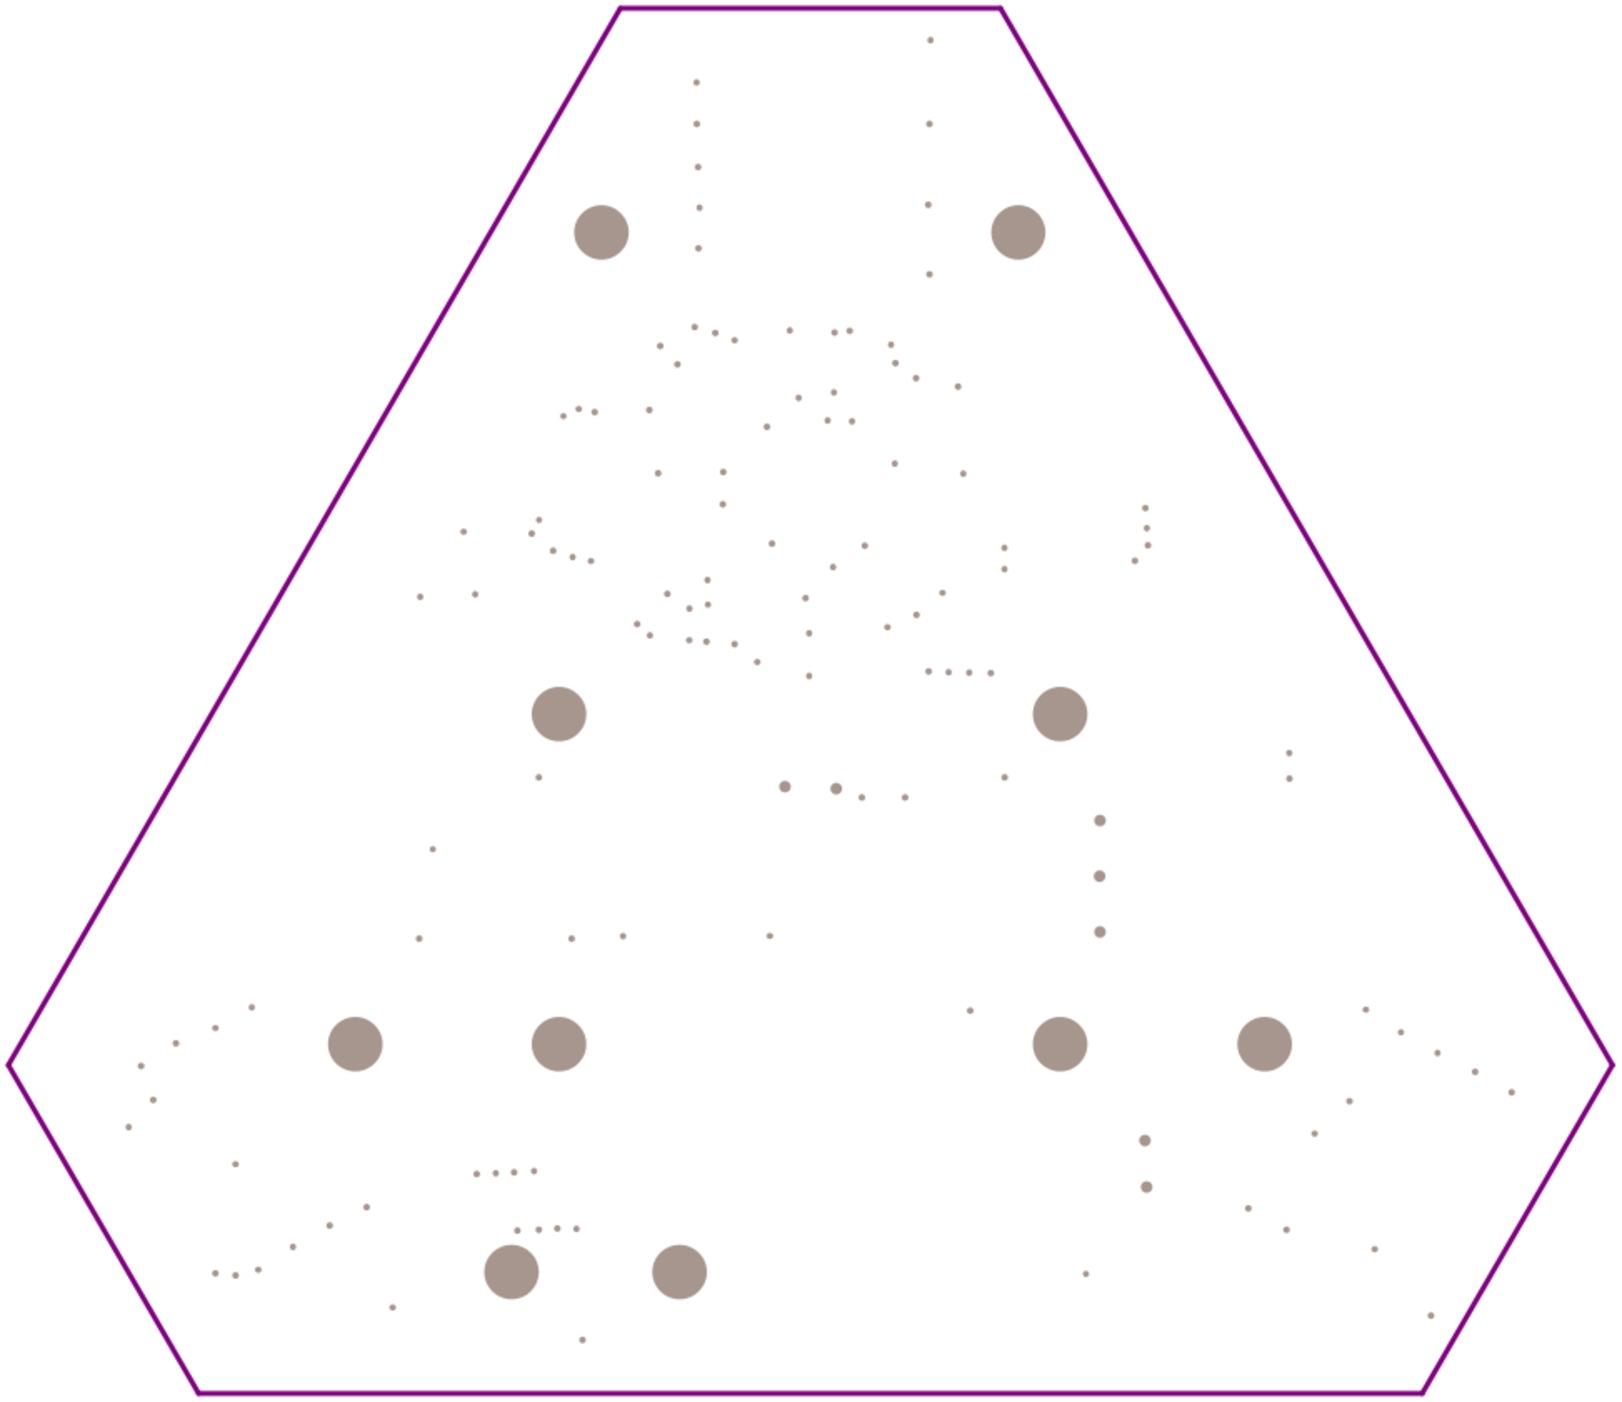
\includegraphics[height=320px]{Imagenes/Vectorial/Capitulo5/cngdshape}  
        \caption{cNGD PCB real size shape. 97x84 mm}
        \label{fig:cap5:cngdshape}
\end{figure}

The \ac{CNGD} \ac{PCB} has to implement the whole design described in Section \ref{cap4:sec:cNGD} attending to expand functionality and usability, and reducing size and cost. Since this is key board of the whole system, most part of the weight of the operation requirements relies on it. It must mainly contain the three \ac{RI}s, give support to expansion modules, include the power supply and battery room, programming system, and microcontroller. In addition, it must provide an easy access to the control modules (\ac{LED}s and push buttons) and easy deployment. Regarding its test-bed character, the module must include some kind of anchors to fix it anywhere or encrust some feet. All these features must be achieved keeping size and cost limited, so the module become affordable and valuable. Figure \ref{fig:cap5:cngdshape} shows the \ac{PCB} shape.

Power supply system, $\mu$USB and PGE connector are gathered together as entire interfacing slot at the large edge 2 of the \ac{PCB}. \ac{RI}s are thought to be placed at the three short edges. 434 MHz \ac{RI} at edge 1, 868 MHZ \ac{RI} at edge 2 and 2.4 GHz \ac{RI} at edge 3. Figure \ref{fig:cap5:cngdfront} can give a better view of these ideas.  

The board includes four holes for the battery to be attached. Figure \ref{fig:cap5:headersystem} illustrates the way it works, four legs fix together the board and the batteries-holder.

\begin{figure}[!h]
\centering
   
\subfloat[Footprint.]{\label{fig:cap5:bat2d}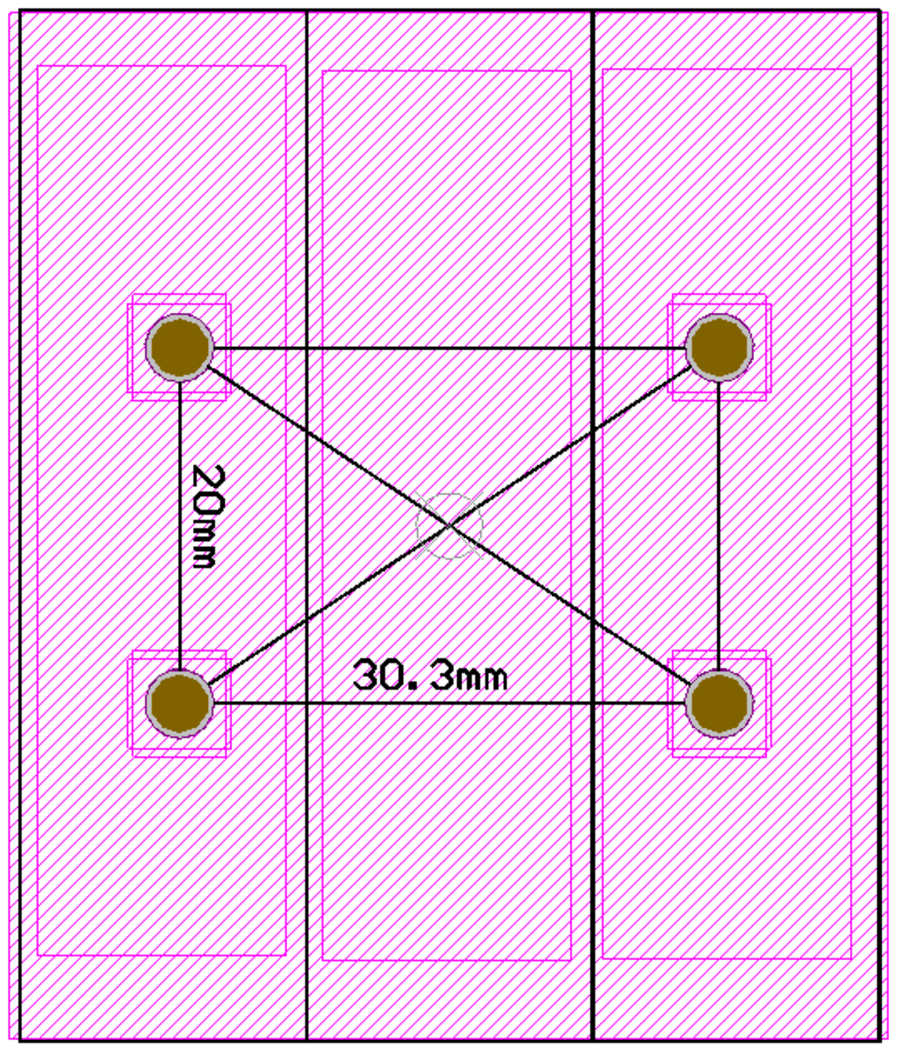
\includegraphics[width=180px]{Imagenes/Vectorial/Capitulo5/bat2d}}  
\qquad
\subfloat[3D model.]{\label{fig:cap5:bat3d}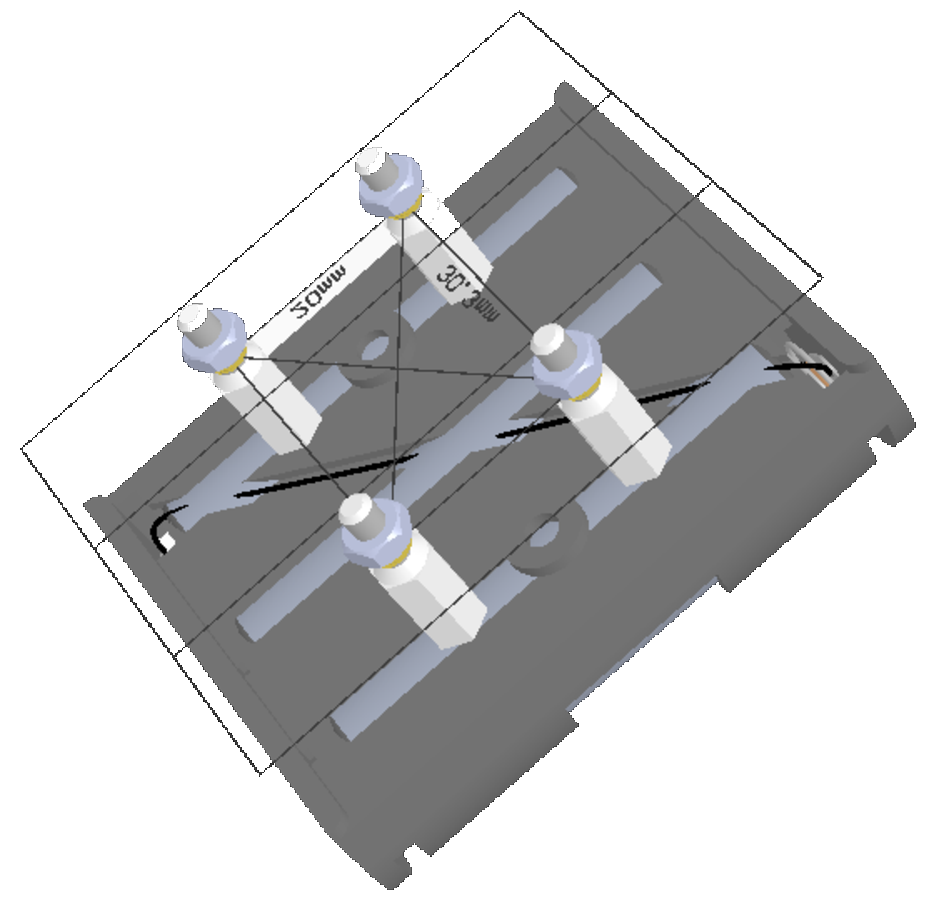
\includegraphics[width=225px]{Imagenes/Vectorial/Capitulo5/bat3d}}
       
\caption{Battery anchorage system.}
\label{fig:cap5:batterysystem}
\end{figure}

Headers module has been placed relying on the large edges 1 and 3, Figure \ref{fig:cap5:cngdheader} shows it. Future expansion modules will be attached to this module through exactly equal headers on them, this way it will be possible to stack several expansion modules ones above others. The headers footprint to include in future expansion modules to fit the design is illustrated in Figure \ref{fig:cap5:headersystem}.

\begin{figure}[!h]
\centering
   
\subfloat[Header detail over cNGD PCB.]{\label{fig:cap5:cngdheader}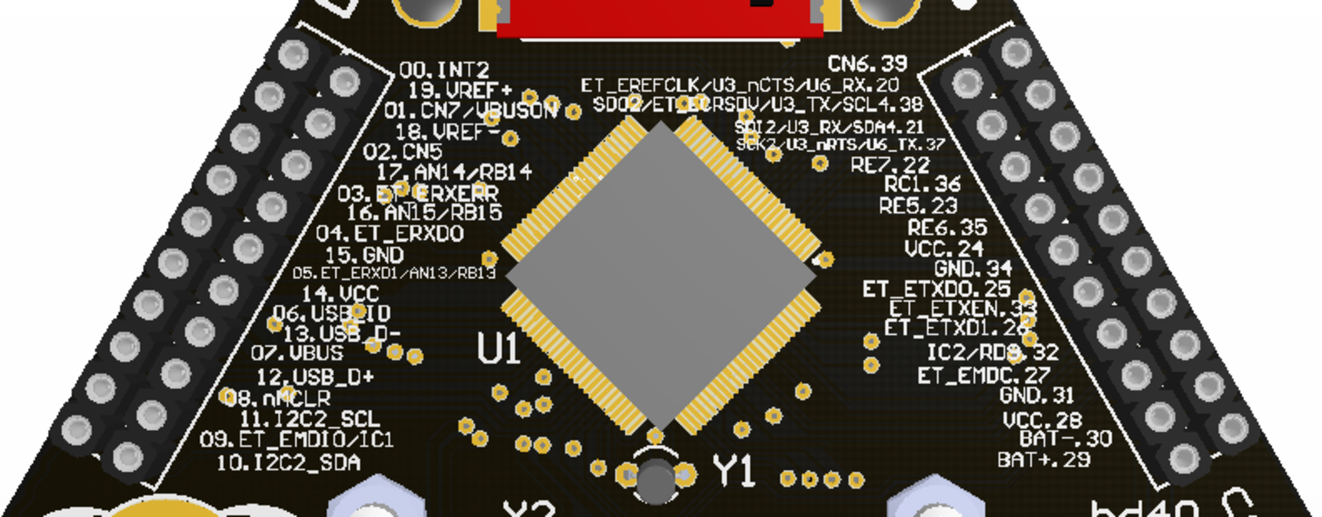
\includegraphics[width=200px]{Imagenes/Vectorial/Capitulo5/headerdetail}}  
\qquad
\subfloat[Header system footprint.]{\label{fig:cap5:headerfootprint}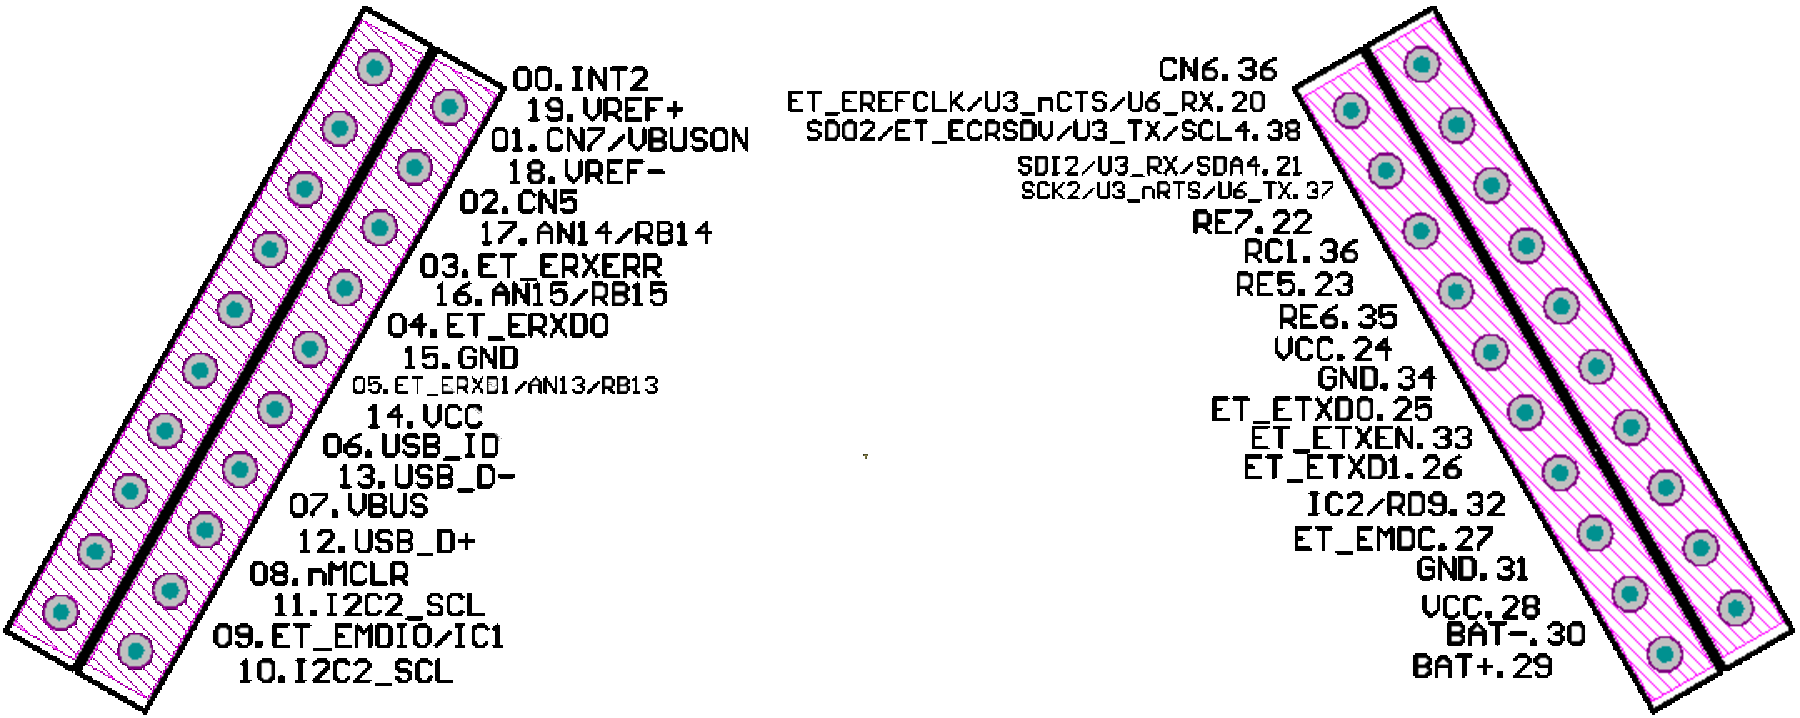
\includegraphics[width=200px]{Imagenes/Vectorial/Capitulo5/headerfooprint}}
       
\caption{40-pin Header system.}
\label{fig:cap5:headersystem}
\end{figure}

The minimum spacing among tracks is set to 0.1 mm around the \ac{MCU} and 0.2 mm in the rest of the layout. Tracks widths vary from 0.2 mm up to 1.2 mm in power tracks. Vias through holes have a 0.4 mm width diameter. Table \ref{tab:ap2:cngdcomponents} at Appendix \ref{ap2:layouts} details the needed components for \ac{CNGD} module.

%-------------------------------------------------------------------
\subsection{Layout}
%-------------------------------------------------------------------
Different layers of the layout can be observed at Appendix \ref{ap2:layouts}. Figures \ref{ap2:cngdtop} and \ref{ap2:cngdbottom} show the top and bottom copper and silkscreens layers respectively.
%-------------------------------------------------------------------
\subsection{Prototype mounting and testing}
%-------------------------------------------------------------------
When prototyping, first part to test is the right operation of the \ac{MCU}. After soldering R4, C2, the reset circuit, PGE module, and the \ac{MCU} itself, the microcontroller is brought under its first programming. For a right operation, is needed a right software configuration of the \ac{MCU} parameters, choosing the internal clock. 

Once the right programming of the \ac{MCU} is tested, the external clocks are mounted and tested by changing the software parameters. After this check, it is time for push buttons and \ac{LED}s, which are tested using test software described in Section \ref{cap6:sec:testBenches}. Rest of decoupling capacitors around the \ac{MCU} can be soldered.

For these already described checkings, power supply from the \ac{ICD} 3 is used. Next step is to mount the power supply system and, using external sources, try the right operation of the mounted modules. Since $\mu$USB takes part of the power supply system, it was checked at this stage. A basic test for the \ac{USB} was included at the firmware.  
 
At this point, the need of debugging traces arises to keep on mounting the device. A serial communication interface is required, and since the used firmware already supports for RS-232 communication, the rs232SHIELD is mounted and used. To read more details about this mounting, go to Section \ref{cap5:sec:rs232shield}. Headers must be soldered on the board to use this shield.

Last modules to try are the \ac{RI}s. One by one, they are added to the \ac{CNGD} and checked. The chosen firmware offers several radio tests for general \ac{TX}/\ac{RX}, handshaking, channel switching. The \ac{RI}s can be tested in conjunction with the equivalent \ac{RI}s at the \ac{FCD}. At this point, it is possible to check the proper operation for the software controlled switches that enable power to the \ac{RI}s. Basic tests have been specifically developed to check this function.

%-------------------------------------------------------------------
\subsection{Final result}
%-------------------------------------------------------------------
\begin{figure}[!h]
\centering
   
\subfloat[Top view.]{\label{fig:cap5:cngdfront}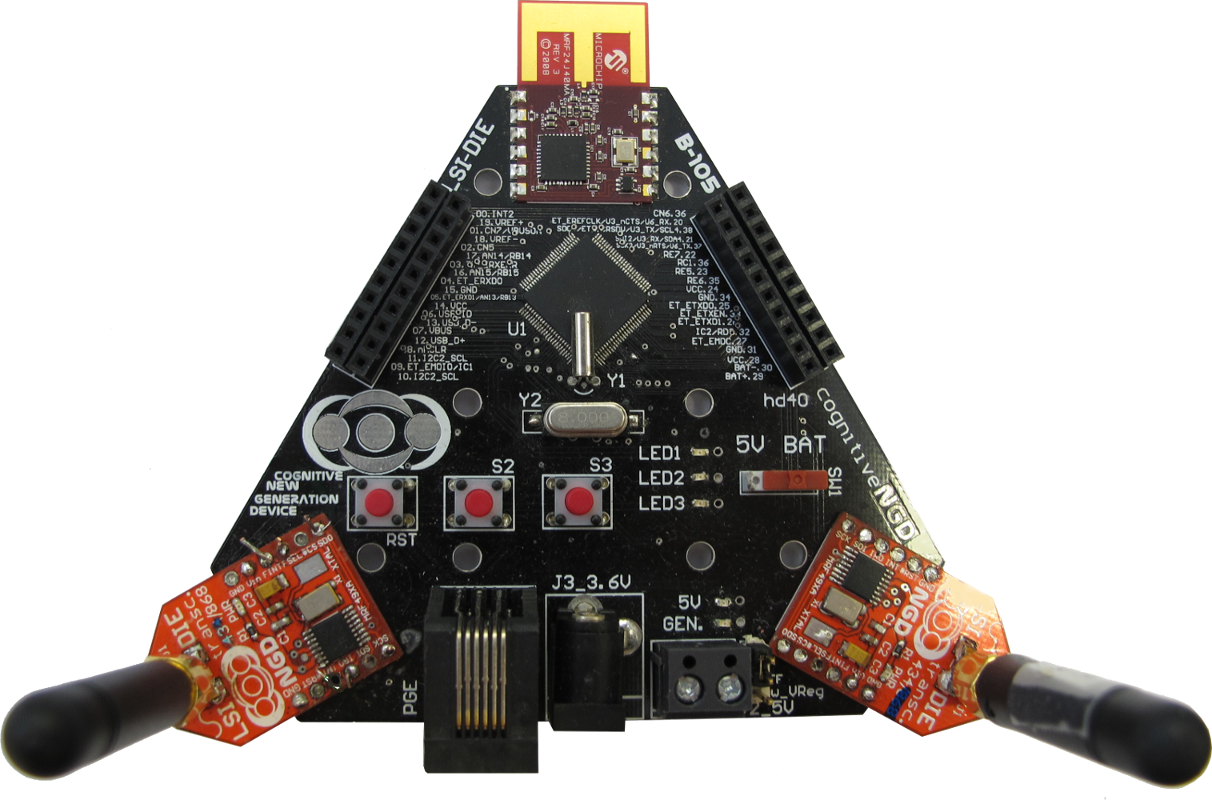
\includegraphics[width=0.6\textwidth]{Imagenes/Bitmap/Capitulo5/cngdtop}}  
\qquad
\subfloat[Bottom view.]{\label{fig:cap5:cngdback}
\includegraphics[width=0.4\textwidth]{Imagenes/Vectorial/Todo}}
       
\caption{Detailed view of the cNGD module.}
\label{fig:cap5:cngd}
\end{figure}

%-------------------------------------------------------------------
\section{Serial Communication Board - rs232SHIELD}
%-------------------------------------------------------------------
\label{cap5:sec:rs232shield}
%-------------------------------------------------------------------

\begin{figure}[!h]
        \centering
		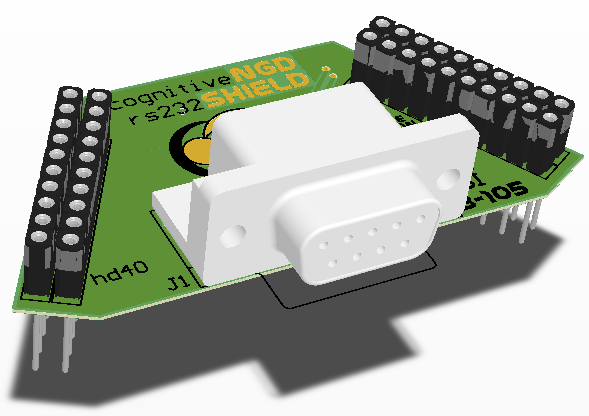
\includegraphics[width=0.6\textwidth]{Imagenes/Bitmap/Capitulo5/rs2323d}  
        \caption{rs232SHIELD 3D model.}
        \label{fig:cap5:rs2323dmodel}
\end{figure}

%-------------------------------------------------------------------
\subsection{Description}
%-------------------------------------------------------------------
This module is an expansion board or shield for the \ac{CNGD} module. The \ac{CNGD} sets the interface with the shield over the already described headers. The board shape posses a total size of 67.9x33 mm.

% HABLAR DEL ENCAPSULADO DEL MAX3232 y de los headers que incluye
The \ac{RX} signal is shorted to pin 21 and \ac{TX} signal to pin 38.

In addition, the module contains a RS-232 female connector to be connected to the computer or other device. Minimal track spacing is set to 0.2 mm while the tracks width is from 0.2 mm to 1.2 mm on power tracks. Vias keep set to a 0.4 mm diameter. Table \ref{tab:cap5:rs232components} at Appendix \ref{ap2:layouts} details the components needed for this module. 

%-------------------------------------------------------------------
\subsection{Layout}
%-------------------------------------------------------------------
Different layers of the layout can be observed at Appendix \ref{ap2:layouts}. Figures \ref{ap2:rs232top} and \ref{ap2:rs232bottom} show the top and bottom copper and silkscreen layers respectively.
%-------------------------------------------------------------------
\subsection{Prototype mounting and testing}
%-------------------------------------------------------------------
This module offers simplicity and does not require for much testing. Basically, the whole module is properly soldered and plugged into the \ac{CNGD} headers. Firmware must be configured to debug over the UART number 3. 

Connecting the RS-232 connector to a computer and with a suitable software, such as Minicom\footnote{Minicom is a text-based modem control and terminal emulation program for Unix-like operating systems. A common use for Minicom is when setting up a remote serial console.}, and configuring properly the communication parameters, is enough to receive data from the running application.

Serial communication parameters can be changed at the firmware configuration. However, a standard configuration is as follows: 
\begin{itemize}
\item Bit rate: 115200 bits/s
\item Bits per framing: 8 bits
\item Parity: No
\item Stop bits: 1 bit
\end{itemize}

%-------------------------------------------------------------------
\subsection{Final results}
%-------------------------------------------------------------------

\begin{figure}[!h]
\centering
   
\subfloat[Top view.]{\label{fig:cap5:rs232front}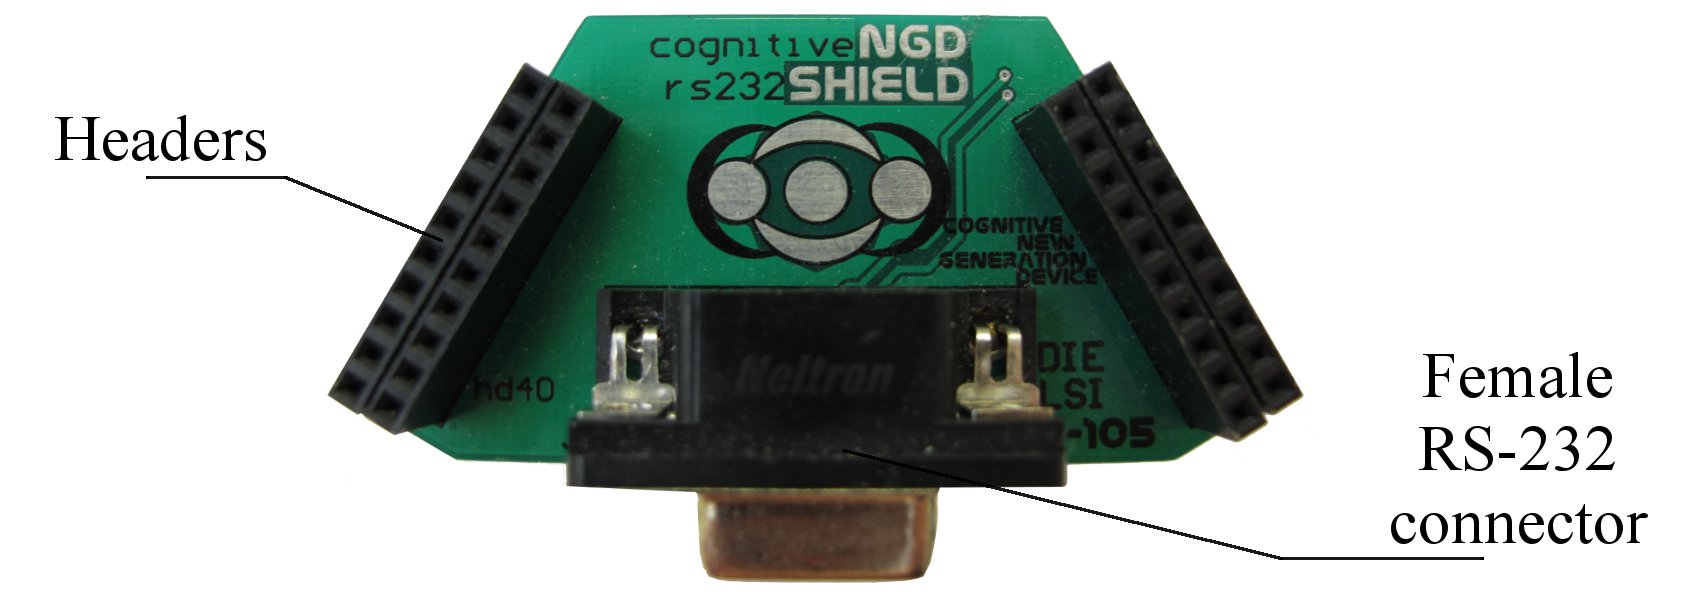
\includegraphics[width=0.4\textwidth]{Imagenes/Bitmap/Capitulo5/rs232top}}  
\qquad
\subfloat[Bottom view.]{\label{fig:cap5:rs232back}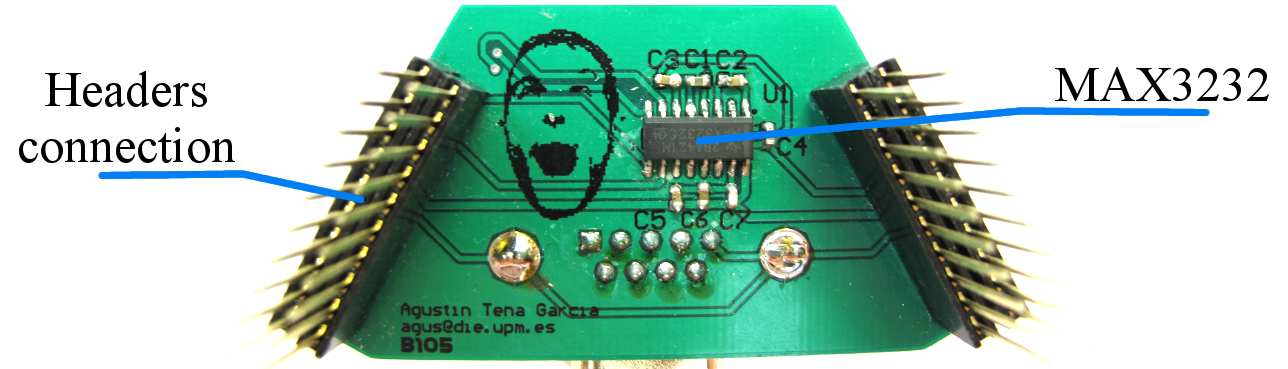
\includegraphics[width=0.4\textwidth]{Imagenes/Bitmap/Capitulo5/rs232bottom}}
       
\caption{Detailed view of the rs232SHIELD module.}
\label{fig:cap5:rs232}
\end{figure}

%-------------------------------------------------------------------
\section{Battery charger - chargerSHIELD}
%-------------------------------------------------------------------
\label{cap5:sec:chargerShield}
%-------------------------------------------------------------------

\figura{Bitmap/Capitulo5/charger3d}{width=0.6\textwidth}{fig:cap5:charger3dmodel}%
{chargerSHIELD 3D model.}

%-------------------------------------------------------------------
\subsection{Description}
%-------------------------------------------------------------------
This module is also a shield for the \ac{CNGD} module. The \ac{CNGD} sets the interface with the shield over the known expansion headers. This sield shares the same shape than rs232SHIELD.

Battery positive pole is accessible at the header on pin 29, negative pole is at pin 30. These two pins are linked to the circuit. Apart from this interface, the charger encrusts a terminal block to connect a external 12V source. This source must be capable to provide up to 500 mA.

Current version of the charger does not include any heat dissipater. Tests showed that not heat dissipater was required for the current configuration. Any change over the resistors configuration must consider the overheating possibility on LM317AMDT component. Thus a heat dissipater could be needed.

Minimal track spacing is set to 0.2 mm while the tracks width is is from 0.2 mm to 1.2 mm on power tracks. Vias posses a minimum through hole of 0.4 mm diameter. Table \ref{tab:ap2:chargercomponents} at Appendix \ref{ap2:layouts} details the components needed for this module. 

%-------------------------------------------------------------------
\subsection{Layout}
%-------------------------------------------------------------------
Different layers of the layout can be observed at Appendix \ref{ap2:layouts}. Figures \ref{ap2:chargertop} and \ref{ap2:chargerbottom} show the copper and silkscreen layers top and bottom respectively.
%-------------------------------------------------------------------
\subsection{Prototype mounting and testing}
%-------------------------------------------------------------------
This module required for a lot of initial debugging, it was needed the use of a breadboard to mount parts of the module in parallel to compare behaviors. It is important to notice that some currents on the circuit are up to 250 mA, existing possibilities of malfunctions that make this even higher. It was needed a external power supply with output current indicator and limitation for it. Of course, this module was not initially tested over the \ac{CNGD}, but emulating it just with batteries or a second voltage source.

First part of the chargerSHIELD to try is the LM311 amplifier and surrounding components, LED, R1, R2, and R3. These parts constitute the comparator and with this, the comparator operation intends to be tested. Once this is checked, rest of components are soldered.

At this point, a lot of tests were carried out using different voltages and number of batteries to calibrate the system. The goal was to adjust the current over the batteries to a proper level, measure charging times and the proper operation of the notification \ac{LED}. R1, R2, R3, and R5 were finally set to their current value. Having this task achieved, external controlled source was swapped by a commercial 12V adapter and its proper operation was proved. 

Once the chargerSHIELD showed a proper operation it was tested over the \ac{CNGD}.
%-------------------------------------------------------------------
\subsection{Final results}
%-------------------------------------------------------------------

\begin{figure}[!h]
\centering
   
\subfloat[Top view.]{\label{fig:cap5:chargerfront}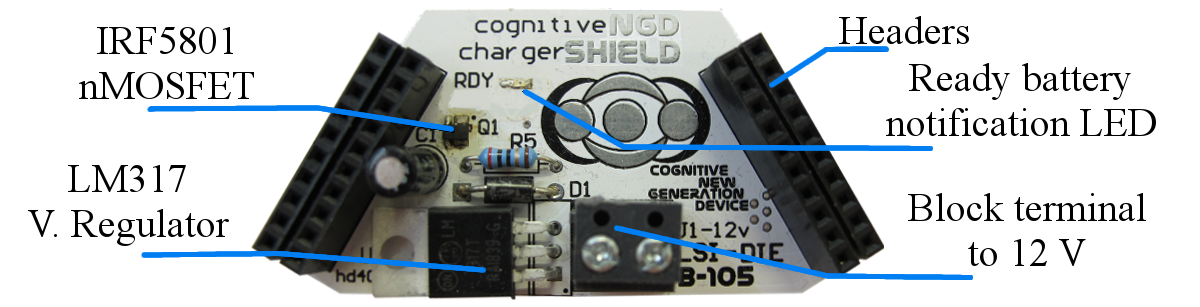
\includegraphics[width=0.4\textwidth]{Imagenes/Bitmap/Capitulo5/chargertop}}  
\qquad
\subfloat[Bottom view.]{\label{fig:cap5:chargerback}
\includegraphics[width=0.4\textwidth]{Imagenes/Vectorial/Todo}}
       
\caption{Detailed view of the chargerSHIELD module.}
\label{fig:cap5:charger}
\end{figure}

%-------------------------------------------------------------------
\section{Conclusions}
%-------------------------------------------------------------------
\label{cap5:sec:conclusions}
%-------------------------------------------------------------------

The whole implementation supposes a modular, versatile, functional, and flexible platform for \ac{CWSN} development. \ac{CNGD} module is the main piece, containing the essential functionalities for a \ac{WSN} node. This main part is able to host up to three \ac{RI}s, becoming the only \ac{WSN} platform together with the \ac{FCD} meeting this feature, and the only platform for \ac{WSN}s capable to access three different frequency bands. In addition, the \ac{CNGD} accepts attachable modules that brings up new functionalities without requiring a new complete design. An existing, ad-hoc developed, firmware has been used to drive the platform as a design requirement. 

It was needed the development of ad-hoc \ac{RI}s based on MRF49XA transceiver. These developed \ac{RI}s, called $\mu$Trans, operate over the 434 MHz and 868 MHz depending on the impedance matching circuitry and antenna they contain. They employ MiWi protocol and support sleep modes. The firmware employed is already prepared to fully drive these \ac{RI}s. It even includes a single MiWi stack shared by the three possible \ac{RI}s. $\mu$Trans are designed to be soldered into the \ac{CNGD} board and they accept external antennas over a coaxial connector.

Third \ac{RI}, a MRF49J40MA, consist of a commercial option that  operates over 2.4 GHz. It is also MiWi compliant, accepts sleep modes and it is supported by the named firmware. This \ac{RI} is also attached to the \ac{CNGD} by soldering and it contains a \ac{PCB} antenna.

\ac{CNGD} is controlled by a PIC32MX675F256L. A 32-bit, low-power, high performance, 100-pin microcontroller that posses a 64KB \ac{RAM} memory and 256KB flash memory. A larger flash memory pin-compatible \ac{MCU} exists in case of need. The \ac{MCU} enables a clock speed up to 80MHz, including an external 8MHz clock and a low-power 32 KHz \ac{RTCC}. The \ac{MCU} supports sleep modes and it is widely featured.

Power supply encrusted into the \ac{CNGD} has been designed to accept either 5V or 3.3V. 5V can be supplied over a $\mu$USB connector, which also serves as serial interface, or a block terminal. This voltage is lowered down into the board voltage operation, 3.3V, by a buck regulator. 3.3V supply option is thought for portability chances, being possible to use an included 3.6V \ac{NIMH} battery for the board. In addition, it is possible to control, from the \ac{MCU}, the \ac{RI}s power supply. 

\ac{CNGD} offer functionality expansions by use of a pair of 20-pin headers. These headers enable access to general use peripherals and unused pins at the \ac{MCU} for future needed implementations. The board contains three \ac{LED}s and two push buttons apart from the reset push button. These components allow interacting with the application.

It has been also developed an attachable shied for the \ac{CNGD} that enables serial communication over an RS-232 protocol accessing an \ac{UART} available at the header. This serial interface has an easier internal operation that the \ac{USB} option and it is useful for old machines or during the platform developing.
 
A charger shield was also developed in order to get the batteries easily charged through the headers. This charger automatically shut-down the charge current at the batteries when the full charge is detected. It also contains a \ac{LED} that indicates when the battery is full. Current used to charge the battery is fixed and it is set to 200 mA. The charger is prepared to charge batteries from 1V to 5V.

%------------------------------------------------------------------
%\section*{\NotasBibliograficas}
%-------------------------------------------------------------------
%\TocNotasBibliograficas

%Citamos algo para que aparezca en la bibliograf�a\ldots
%\citep{ldesc2e}

%\medskip

%Y tambi�n ponemos el acr�nimo \ac{CVS} para que no cruja.

%Ten en cuenta que si no quieres acr�nimos (o no quieres que te falle la compilaci�n en ``release'' mientras no tengas ninguno) basta con que no definas la constante \verb+\acronimosEnRelease+ (en \texttt{config.tex}).


%-------------------------------------------------------------------
%\section*{\ProximoCapitulo}
%-------------------------------------------------------------------
%\TocProximoCapitulo

%...

% Variable local para emacs, para  que encuentre el fichero maestro de
% compilaci�n y funcionen mejor algunas teclas r�pidas de AucTeX
%%%
%%% Local Variables:
%%% mode: latex
%%% TeX-master: "../Tesis.tex"
%%% End:
